

% Neil Notman's Hons Project

% Notes:

\pagestyle{fancy}

\lhead{Neil Notman}
\rhead{40124066}
\lfoot{Games Development BSc (Hons)}
\cfoot{}
\rfoot{\thepage}
\title{Procedural level generation and dynamic pathfinding a combined approach}
\author{Initial Project Overview\\Neil Notman\\40124066}
\providecommand{\keywords}[1]{\textbf{Keywords---} #1}
\date{}

\sloppy



\renewenvironment{abstract}
  {\small\quotation
  {\bfseries\noindent{\large\abstractname\\\noindent{}}}}
  {\endquotation}


\setlength\parindent{0cm}


\keywords{Level-Generation,Path-Finding,Algorithm,Optimisation}

\subsection{Overview of  Project Content and Milestones}
This project will include research into current practices used in industry for path-finding and level generation with the emphasis being performance based compared against realism. The main milestone for this stage will be coming across a method to integrate both level generation and path-finding into an algorithm which will be carried forward to the development stage.\\

Development of an application which will utilise both level generation and path-finding either by the modification and optimisation of existing approaches or the creation of a new algorithm. The application will allow the user to create various sizes of level and the application will then give a visual representation of both the level and path that has been built.\\

The application will then be optimised and tested against some of the methods researched with the aim to show that a combined approach may achieve better results in a similar or faster run time with the paths created being checked for mistakes or inconsistencies based on various sanity checks (no path nodes on areas that should not be traversable such as extreme slopes or dips in the level).\\

Creation of a report that contains all project information and related work with a detailed analysis and testing of the approach used to provide an evaluation of the solution using performance figures to accurately examine the viability of this approach in comparison to the current industry standards and draw a conclusion over the project as a whole.\\

For a more detailed look at the time-line for this project please refer to Figure \ref{gantt}\\

\subsection{The Main Deliverables}
\begin{itemize}
\item A application that will allow the user to create various sizes of level and will give a visual output of the level and path built with a focus on the optimisation techniques used to integrate level generation and path finding.\\
\item A detailed report containing an analysis on the approach taken and a comparison between the solution and other methods used currently using figures from both to evaluate the effectiveness and viability of the approach used.\\
\item Test logs of the finished application and an industry standard practice to allow for an unbiased comparison to be made based on results obtained from these tests when documenting the project.
\end{itemize}

\subsection{Target audience for the deliverables}
The deliverables of this project may be of interest to people involved with both level generation and path finding in the games development industry. Researchers involved in this field may find the report and comparison of techniques used to be of interest. Other people may find this project helpful with regards to optimisation techniques. The main aim of the project  is to show the performance of a combined approach to level generation and path-finding and an evaluation of the quality of paths built. 

\subsection{The work to be undertaken}
\begin{itemize}
\item Research into current industry practices for level generation and path finding to allow for visualization of a solution to combine these algorithms.\\
\item Development of the application and chosen approach with a focus on performance while maintaining a level of realism.\\
\item Optimisation of the developed solution and gathering of test data from the solution and an industry approach.\\
\item Creation of a report detailing the approach taken to implementing the project and providing an evaluation between the solution compared to industry practices.  
\end{itemize}
There is a diagram showing expected steps of execution within the application shown at Figure \ref{block}

\subsection{Knowledge and skills required}
To be able to complete the project to a high standard I will first need to research the field’s of both level generation and path finding as a solid knowledge will be needed to create a combined approach. In terms of development further research into optimisation techniques for C++ in Visual Studio will allow for a more polished and better performing solution also as a level of realism will be maintained experience with graphic programming would also benefit the project.  

\subsection{Information sources that provide a context for the project}
The video available at \cite{levels1} gives a few very basic examples of levels that can be generated and also details some methods to define areas within a level(slopes,walls,and others) this definition of areas within a level could be used for testing the path finding within the project and may give a basic concept on how to generate content within the level produced in relation with the project.\\

The paper\cite{paths1} analyses various path-finding algorithms however the purpose of their project was to look at an alternative approach to the A* path finding algorithm.  Use of concepts such as map abstraction could be of interest to this project as it would allow a way to break the level into chunks which can then be processed individually by a path finding algorithm.\\

The textbook for level generation \cite{levels2} Provides extensive research into procedurally generated content in games from grid based levels to full landscapes there are multiple approaches detailed within the textbook that can provide a basis to generate a level within the project.\\

\textbf{Previous honours projects to note}\newline
This paper\cite{honours} analyses various path finding algorithms and discusses at optimisation options this will be the inspiration for optimising the project and will give a wide variety of path finding algorithms to research going forward.\\

For a timeline of research into path finding algorithms please refer to Figure \ref{timeline}

\subsection{The importance of the project}
This project is important as it will seek to integrate level generation and path finding which could allow for faster loading times in games while reducing the storage space taken by a game. When comparing the difference between developed solution and current industry practices - if the solution proves to be better in terms of performance and the quality of the path built is of a suitable standard for the complexity of the level that is generated.   

\subsection{The key challenges to be overcome}
\begin{itemize}
\item  Research of a variety of level generation and path-finding techniques to gain knowledge and propose a viable solution for development.\\
\item Development of  an application that will use the envisioned solution and give a visual output to the user of both level and path built.\\
\item Research into a way of determining the quality of path finding and level generation techniques.\\
\item Writing of a detailed report that will clearly explain the solution chosen and give a view into past work done within this field then the report will provide an unbiased comparison between the approach and current industry practices to evaluate the project in terms of the quality the path built when compared to the complexity of the level generated.
\end{itemize}

\begin{figure}[ht!]
	\begin{tabular}{ |p{5cm}|p{3.5cm}|p{0.8cm}|}
	\hline
            Creator & Method & Year \\
             \hline
            Dijkstra \cite{dijkstra} & Graph searching & 1959 \\
            \hline
            Goodchild \cite{goodchild} & Orthagonal and diagonal movement & 1977\\
            \hline
            Huber and Church \cite{huber} & analysis of neighboring cells & 1985\\
            \hline
            Eastman \cite{eastman} & Pushbroom procedure & 1989\\
            \hline
            Lombard and Church \cite{lombard} & GSP(Gateway-shortest-path) & 1993\\
            \hline
            Mcilhagga \cite{mcilhagga} & Fixed cost distance & 1997\\
            \hline
            Andrea Califano \cite{califano} & Splash algorithm & 2000\\ 
            \hline
\end{tabular} 
	\caption{A time-line of path finding algorithms}	 \label{timeline} \cite{Time}
\end{figure}

\begin{landscape}
\begin{figure}[ht!]
	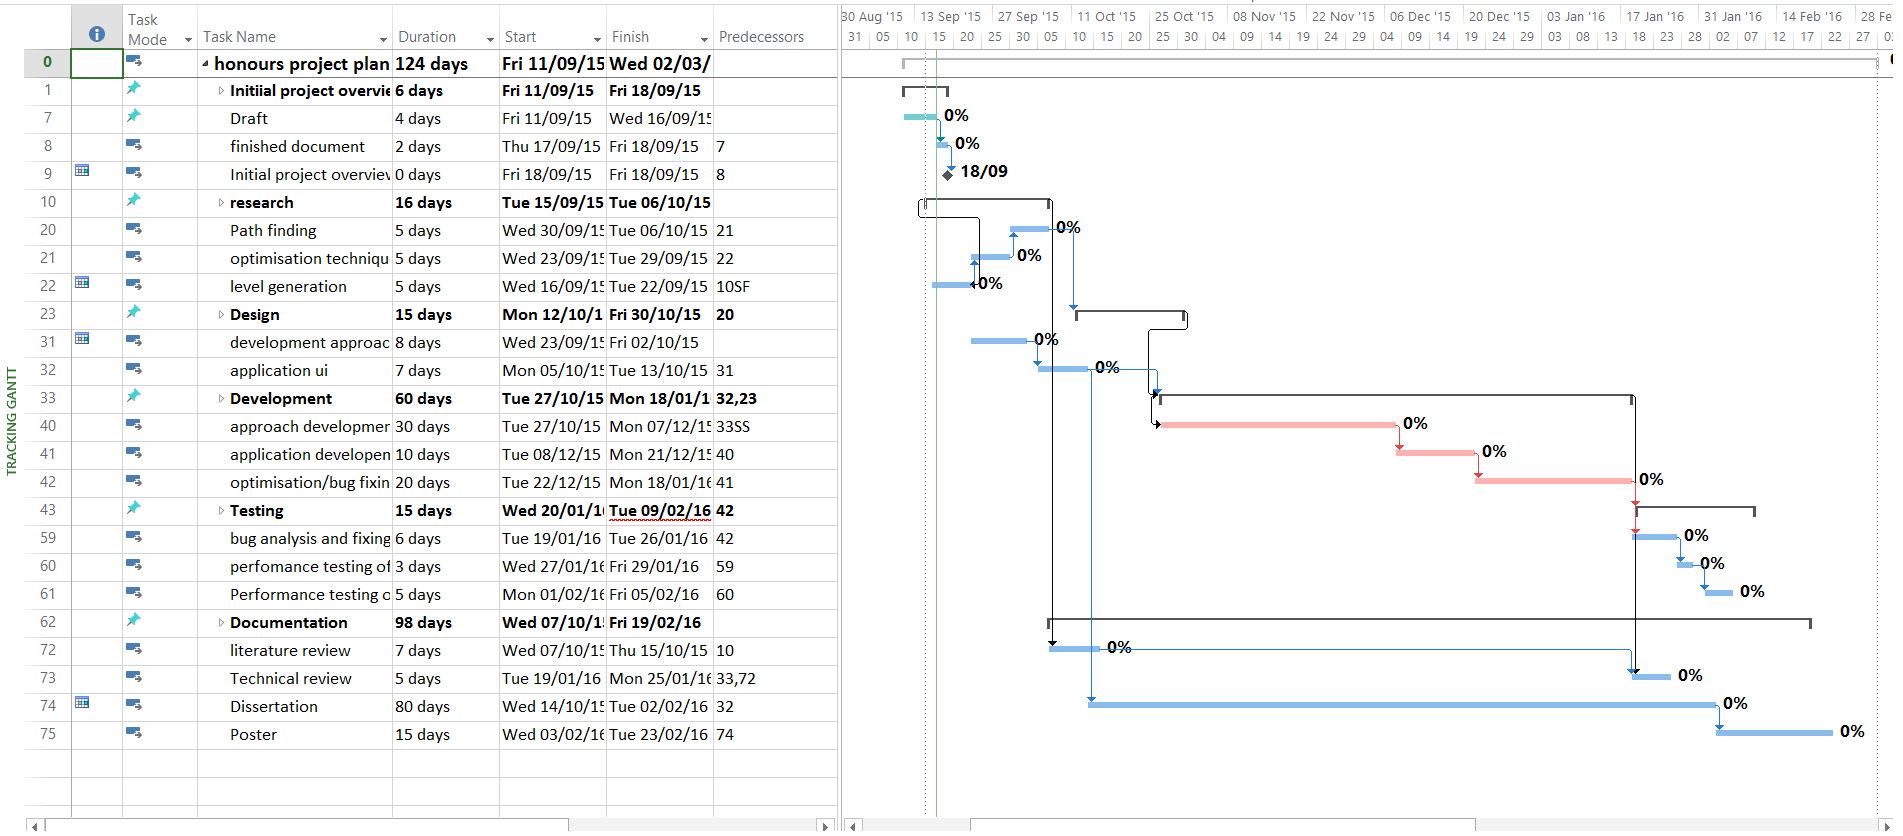
\includegraphics[width=1.5\textwidth]{images/project-plan}
	\caption{An image of the project gantt chart	 \label{gantt}}
\end{figure}
\end{landscape}



\begin{figure}[ht!]
	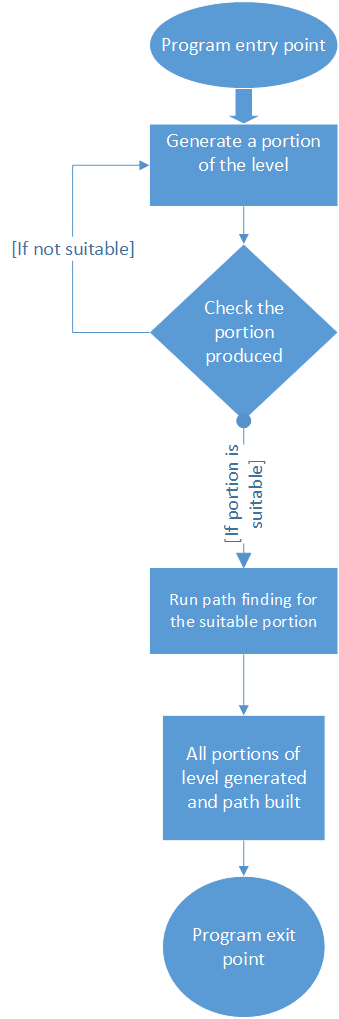
\includegraphics[width=1.0\textwidth, height =1.4\textwidth]{images/block-diagram}
	\caption{This shows how the program will execute	\label{block}}
\end{figure}





